\hypertarget{wusatowski-spreading-model-for-groove-rolling}{%
\section{Wusatowski Spreading Model for groove
rolling}\label{wusatowski-spreading-model-for-groove-rolling}}

\hypertarget{wusatowskis-spread-equation}{%
\subsection{Wusatowski's spread
equation}\label{wusatowskis-spread-equation}}

Wusatowski proposed the following equation for estimation of spreading
in flat rolling:

\begin{Shaded}
\begin{Highlighting}[]
\NormalTok{    \textbackslash{}beta = \textbackslash{}frac\{b\_1\}\{b\_0\} = a \textbackslash{}times c \textbackslash{}times d \textbackslash{}times f \textbackslash{}times \textbackslash{}gamma\^{}\{{-}w\}}
\end{Highlighting}
\end{Shaded}

\(`\gamma = \frac{h_1}{h_0}`\) is the compression. \(`h`\) and \(`b`\)
are height and width of the workpiece with the indices 0 and 1 denoting
the incoming respectively the outgoing profile. \(`a`\), \(`c`\),
\(`d`\) and \(`f`\) are correction coefficients for temperature,
velocity, material and friction, respectively.

\(`c`\) can be assumed as below in dependence on the velocity \(`v`\):

\begin{Shaded}
\begin{Highlighting}[]
\NormalTok{    c = \textbackslash{}left({-}0.002958 + 0.00341 \textbackslash{}gamma \textbackslash{}right) v + 1.07168 {-} 0.10431 \textbackslash{}gamma}
\end{Highlighting}
\end{Shaded}

\(`w`\) is the spread exponent, many different expression were given by
various authors for its value. The original expression by Wusatowski is:

\begin{Shaded}
\begin{Highlighting}[]
\NormalTok{    w = 10\^{}\{ {-}1.269 \textbackslash{}left( \textbackslash{}frac\{h\_0\}\{2 R\} \textbackslash{}right)\^{}\{0.56\} \textbackslash{}frac\{b\_0\}\{h\_0\} \}}
\end{Highlighting}
\end{Shaded}

\(`R`\) is the roll radius.

\hypertarget{equivalent-rectangle-approach}{%
\subsection{Equivalent rectangle
approach}\label{equivalent-rectangle-approach}}

Wusatowskis spreading model was originally built for flat rolling. A
common approach for groove rolling is to calculate some equivalent
rectangular profile to be able to use flat rolling models.

The figure below shows 3 variants of calculating an equivalent rectangle
of a profile.

\begin{figure}
\centering
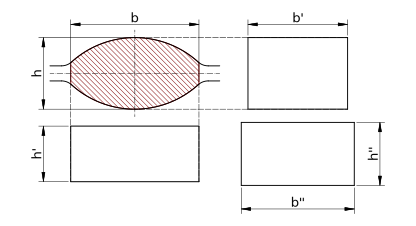
\includegraphics{equivalent_rectangle.svg}
\caption{equivalent rectangle}
\end{figure}

The first variant is to keep the width constant and calculate the height
\(`h'`\) so that the cross section \(`A`\) is equal:

\begin{Shaded}
\begin{Highlighting}[]
\NormalTok{    h\textquotesingle{} = \textbackslash{}frac\{A\}\{b\}}
\end{Highlighting}
\end{Shaded}

The second variant is to keep the height constant and calculate the
width \(`b'`\) so that the cross section \(`A`\) is equal:

\begin{Shaded}
\begin{Highlighting}[]
\NormalTok{    b\textquotesingle{} = \textbackslash{}frac\{A\}\{h\}}
\end{Highlighting}
\end{Shaded}

Both represent the geometry of the profile poorly. A better way is to
keep the aspect ratio equal:

\begin{Shaded}
\begin{Highlighting}[]
\NormalTok{    h\textquotesingle{}\textquotesingle{} = \textbackslash{}sqrt\{\textbackslash{}frac\{A h\}\{b\}\}}
\end{Highlighting}
\end{Shaded}

\begin{Shaded}
\begin{Highlighting}[]
\NormalTok{    b\textquotesingle{}\textquotesingle{} = \textbackslash{}sqrt\{\textbackslash{}frac\{A b\}\{h\}\}}
\end{Highlighting}
\end{Shaded}

This variant is used in the current implementation. So \(`h`\) and
\(`b`\) in Wusatowski's model are replaced with \(`h''`\) and \(`b''`\).
In the end, \(`b_1`\) can be obtained from \(`b_1''`\) by:

\begin{Shaded}
\begin{Highlighting}[]
\NormalTok{    b\_1 = \textbackslash{}frac\{b\_1\textquotesingle{}\textquotesingle{} h\_1\}\{h\_1\textquotesingle{}\textquotesingle{}\}}
\end{Highlighting}
\end{Shaded}

\hypertarget{references}{%
\subsection{References}\label{references}}

\begin{itemize}
\tightlist
\item
  Wusatowski, Z.: Fundamentals of Rolling, Pergamon Press, 1969
\item
  Hensel, Spittel: Kraft- und Arbeitsbedarf bildsamer
  Formgebungsverfahren, Deutscher Verlag für Grundstoffindustrie,
  Leipzig, 1978
\end{itemize}
